% !TEX root = diplomarbeit.tex
\chapter{Einleitung}
\renewcommand{\kapitelautor}{Autor: Markus Kaiser}

%%%%%%%%%%%%%%%%%%%%%%%%%%%%%%%%%%%%%%%%%%%%%%%%%%%%%%%%%%%%%%%%%%%%%%%%%%%%%%%
\section{Projektidee}
Die Idee des Projektes ist die Entwicklung einer Konzeptstudie eines innovativen Logistiksystems, das sich durch die Verwendung eines Multicopters auszeichnet.
Für den Entwicklungsprozess im Zuge der Diplomarbeit wurde die Gastronomie als Einsatzbereich gewählt. Diese Wahl ermöglicht zum einen
ein konkreteres Formulieren der Ziele und zum anderen eine einheitliche Vision innerhalb des Teams.

Der innovative Aspekt des Projekts wird insofern abgedeckt, dass die Entwicklung des Systems so durchgeführt wird,
dass es auch in anderwärtigen Bereichen der Logistik, wie beispielsweise der Lagerverwaltung, eingesetzt werden kann.

Das System setzt sich aus den folgenden drei Komponenten zusammen:

\begin{itemize}
  \item Multicopter
  \item Firmware
  \item Digitale Speisekarte
\end{itemize}

\begin{figure}[H]
  \begin{centering}
  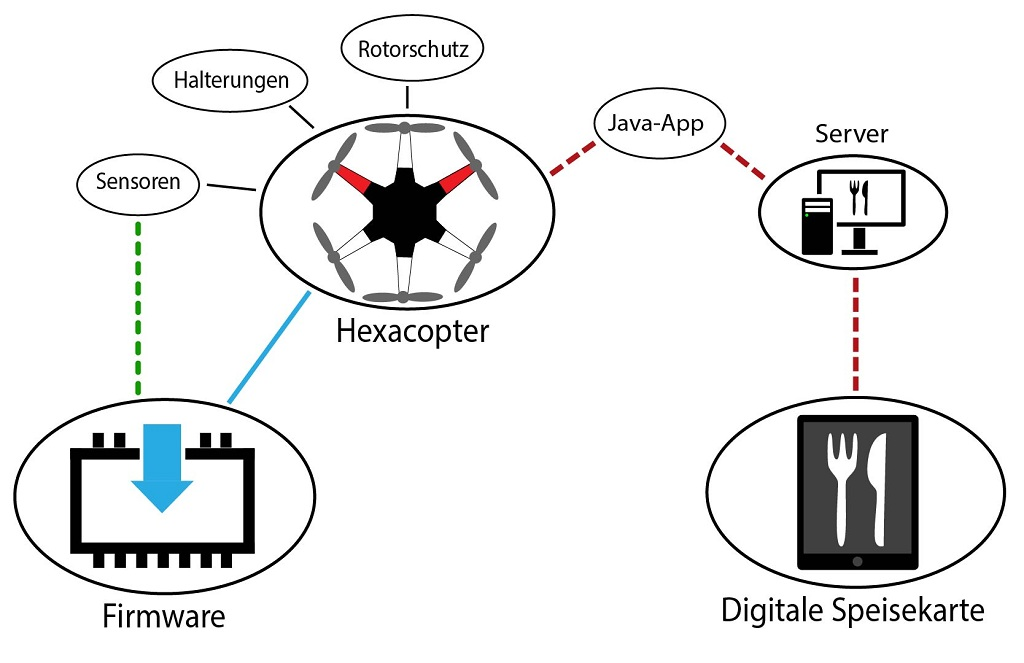
\includegraphics[width = 0.9\textwidth]{Bilder/systemblockbild.jpg}
  \par\end{centering}
  \caption{Systemblockbild}
  \label{Systemblockbild}
\end{figure}

Der Multicopter ist die zentrale Komponente des Projekts. Er ist für den selbstständigen Transport von Objekten zuständig
und muss somit flugfähig und im Stande sein, Unfälle zu verhindern. Sensoren, die mittels eigens angefertigter Halterungen
am Multicopter befestigt sind, kommunizieren mit der Firmware.

Die Firmware regelt alle logischen Prozesse des Systems. Sowohl die Steuerung des Multicopters, als auch der
Austausch von Daten fällt unter diese Kategorie. Befehle erhält sie unter anderem von der Speisekarte, mit der sie über
einen Server, beziehungsweise einer weiteren Anwendung, kommuniziert.

Die digitale Speisekarte ist indirekt die externe Steuereinheit des Multicopters und zugleich die Komponente,
die das System für den Einsatz in der Gastronomie auszeichnet. Sie automatisiert Vorgänge eines gastronomischen
Betriebs und wandelt Nutzereingaben in Befehle für den Muticopter um.

%%%%%%%%%%%%%%%%%%%%%%%%%%%%%%%%%%%%%%%%%%%%%%%%%%%%%%%%%%%%%%%%%%%%%%%%%%%%%%%
\section{Ausgangssituation}
  In den folgenden Absätzen wird beschrieben, wie die Idee von Hovering Steward, dem autonom fliegenden Kellner,
  entstanden ist und womit sich die ersten Recherchen zu Beginn des Projektes beschäftigt, beziehungsweise
  welche Ergebnisse diese hervorgebracht haben.

  \subsection{Ideenfindung}
  Ihren Anfang fand die Idee im Projektmanagement Unterricht. Klasseninterne Teams mussten ein fiktives Projekt erfinden, um auf Basis dieses
  Projektmanagementpläne zu erstellen. Es entstand "Fluorescent Bakery", eine Bäckerei, die fluoreszierende Cupcakes verkauft.
  Bei dem Gedanken diese Idee für die Diplomarbeit weiterzuverwenden, entstand das Grundgerüst für die Idee, wie sie schlussendlich im Projekt aussah. Der Ansatz hierfür war,
  einen nicht menschlichen Kellner zu erschaffen, der, selbstprogrammiert, die Aufgaben einer Bedienung in einem Restaurant übernimmt.
  So entstand "Hovering Steward - der autonom fliegende Kellner", ein dreidimensionales "Tracking-System", welches eine Drohne in einem Raum die Aufgaben eines Kellners durchführen lässt.
  Das Projekt erhielt später noch eine weitere Komponente, nämlich eine digitale Speisekarte, um das automatische System zu erweitern.

  \subsection{Stand der Technik}
  \subsection*{Themenrestaurants}

  \begin{itemize}
    \item \textbf{Disaster Café}

    Das Themenrestaurant {Disaster Café\cite{disastercafe}} in Spanien bietet Gästen die Erfahrung ihr Essen bei einem Erdbeben
    der Stärke 7.8 zu sich zu nehmen.

    \item \textbf{Das stille Örtchen - Modern Toilet}

    Eingerichtet wie eine Toilette können Gäste des {Modern Toilet\cite{moderntoilet}} in Japan ihre Speisen in einem gewohnten Umfeld genießen.

    \item \textbf{Affen-Kellner}

    {Eine kleine Taverne in Japan\cite{affenkellner}} besitzt zwei kleine Affen, die Tätigkeiten wie das Servieren von Getränken oder Handtüchern
    für den Inhaber übernehmen. Sie verstehen sogar, welche Getränke ein Gast bestellt.

    \item \textbf{{The Royal Dragon\cite{royaldragon}}}

    Neben Rollschuh fahrenden Kellnern verfügt das weltweit größte Restaurant für Meeresfrüchte eine
    Art Seilbahn, mit der ein Kellner "fliegend" das Essen serviert.

    \item \textbf{Dinner in the Sky}

    Bei {Dinner in the Sky\cite{dinnerinthesky}} werden die Gäste samt Tisch und kleiner Küche von einem Kran 50 Meter
    in die Luft gezogen, wo dann gespeist wird.

    \item \textbf{{Dinner in the Dark\cite{dinnerinthedark}}}

    In diesem Themenrestaurant verbringen die Gäste ihren Aufenthalt im Dunkeln. Einzig und allein die
    Kellner können mittels Nachtsichtbrille etwas sehen.

  \end{itemize}

  \subsection*{Multicopter in der Gastronomie}
  \begin{itemize}
      \item \textbf{{Infinium-Serve\cite{infiniumserve}}}

      Das Unternehmen Infinium-Robotics hat ein System entwickelt, welches Gästen eines Restaurants
      das Essen mittels Hexacopter serviert.

      \item \textbf{iTray}

      {iTray\cite{itray}}, ein Projekt aus London, nutzt kleine Drohnen, um Sushi an die Tische der Gäste zu bringen.
      Die Drohnen werden über ein Remote-Wi-Fi-System gesteuert.

  \end{itemize}

  \subsection*{Multicopter Projekte}
  \begin{itemize}
      \item \textbf{ETH Flying Machine Arena}

      Die {Flying Machine Arena\cite{eth}} ist ein portables System, welches einen virtuellen Raum mit den Maßen 10x10x10 Meter aufbaut, in welchem
      Objekte mit hoher Präzision erkannt und verfolgt werden können. Das System ist für Experimente mit autonom fliegenden Hexacoptern
      gedacht, die sich in diesem virtuellen Raum über drahtlose Kommunikation orientieren können.

      \item \textbf{Lily}

      {Lily\cite{lily}} ist eine selbstständig fliegende Drohne mit eingebauter Kamera. Ihr Zweck ist, dass sie den Benutzer auf seinem Weg verfolgt.
      Sie wird dafür einfach in die Luft geworfen, worauf sie sich stabilisiert. Danach folgt sie dem Benutzer in einem festgelegten Abstand, solange dieser ein für Lily
      vorgesehenes Armband trägt und filmt mit einer HD Kamera alles mit.

      \item \textbf{DHL Paketcopter}

      Der {DHL Paketcopter\cite{dhl}} ist ein Innovationsprojekt der DHL, bei dem ein Paket per Drohne zugestellt wird. Die Drohne ist in der Lage große Strecken zu fliegen,
      um somit auch zu schwer erreichbaren Orten zu gelangen, wenn Menschen dazu keine Möglichkeit mehr haben. Auf der Insel Juist wird sie beispielsweise als
      Medikamentenversorger verwendet, da am Wochenende keine Lieferungen per Schiff auf die Insel zugestellt werden.

      \item \textbf{Ambulance Drone}

      Die {Ambulance Drohne\cite{ambulancedrone}} ist ein Projekt, welches auf der TU Delft entwickelt wird. Das Besondere an dieser Drohne ist, dass sie einen eingebauten Defibrillator hat, welcher
      sich per Fernverbindung von einem Rettungshelfer bedienen lässt, obwohl dieser nicht anwesend ist. Die Ambulance Drohne fliegt mit einer Höchstgeschwindigkeit von bis zu
      100 Stundenkilometer und kann somit in einem Notfall schnell die Unfallstelle erreichen.

      \item \textbf{Gimball}

      {Gimball\cite{gimball}} ist der weltweit erste fliegende Roboter, der immun gegen Kollistionen ist. Seine Konstruktion besteht aus einem kugelförmigen Gerüst, in dem die Drohne
      aufgehängt ist, und sich anhand von Gelenken trotzdem frei darin bewegen kann. Die Kugel fängt Stöße ab, wodurch die Drohne ungehindert an schwer erreichbare
      Orte gelangt.

  \end{itemize}

%%%%%%%%%%%%%%%%%%%%%%%%%%%%%%%%%%%%%%%%%%%%%%%%%%%%%%%%%%%%%%%%%%%%%%%%%%%%%%%
\section{Team und Aufgabenverteilung}
  \subsection*{Markus Kaiser}
  \textbf{Projektleitung und Marketing}

  Markus Kaiser leitete das Team Hovering Steward und war somit für das Projektmanagement und
  die organisatorischen Aspekte verantwortlich. Neben dieser Hauptrolle zählte außerdem das Marketing
  zu seinen Aufgabenbereichen, was speziell die Entwicklung des Blogs anbelangte. Durch seine Kenntnisse
  in der Webentwicklung stellte er mit dem Blog eine wichtige Schnittstelle zur Außenwelt her.

  \subsection*{Lucas Ullrich}
  \textbf{Sensorik \& Firmware}

  Lucas Ullrich war neben seiner Position als Projektleiter Stellvertreter für die Sensorik der Drohne und
  für die Programmierung der Firmware zuständig. Er unterstützte den Projektleiter bei terminlichen Angelegenheiten
  und konnte durch seine Kenntnisse mit der Programmiersprache C eine solide Basis für die Firmware des Mikrocontrollers schaffen.
  Außerdem entwarf er die Schaltpläne und erstellte somit ein Konzept für die Sensorik.

  \subsection*{Christina Bornberg}
  \textbf{Firmware}

  Christina Bornberg fungierte als Firmware Entwicklerin des Teams. Durch ihre Interesse an der Programmierung von Drohnen
  und bereits gesammelten Erfahrung mit der Programmierung von C konnte sie gemeinsam mit Lucas Ullrich die erarbeiteten Konzepte hinter
  dem automatisierten Flug der Drohne in Code realisieren.

  \subsection*{Katharina Joksch}
  \textbf{Webentwicklung}

  Der Aufgabenbereich von Katharina Joksch war die Webentwicklung, genauer gesagt die Programmierung der digitalen Speisekarte.
  Neben der Planung der Datenbank und der sinnvollen Verwendung hilfreicher Frameworks entwickelte sie außerdem eine Java Applikation,
  die die Kommunikation zwischen der digitalen Speisekarte und der Drohne regelte.

  \subsection*{Alexander Punz}
  \textbf{Hardware \& Mechanik}

  Alexander Punz war sowohl für die Hardware, als auch für die Mechanik verantwortlich. Seine Aufgaben waren sowohl die Konzeption
  und Produktion des Rotorschutzes, der einen sicheren Flug der Drohne ermöglichte, als auch die Herstellung diverser Halterungen,
  die für Sensorik, Transport und Flugtests vorausgesetzt waren.

%%%%%%%%%%%%%%%%%%%%%%%%%%%%%%%%%%%%%%%%%%%%%%%%%%%%%%%%%%%%%%%%%%%%%%%%%%%%%%%
\section{Betreuer}
  \subsection*{Mag. Andreas Fink}
  Mag. Andreas Fink stand dem Projektteam als Hauptbetreuer der Abteilung für Informationstechnologie zur Seite.
  Seine objektive Sichtweise auf das Projekt hat dem Team sehr geholfen, den Fokus auf die Ziele zu legen und
  das Projekt in die richtige Richtung zu entwickeln.
  Zusätzlich dazu betreute er individuell Markus Kaiser bei den Aspekten Projektleitung und Marketing.

  \subsection*{DI Herbert Fleck}
  DI Herbert Fleck war Hauptbetreuer der Mechatronik Abteilung des Teams. Er koordinierte den Prozess der Diplomarbeit
  gemeinsam mit Mag. Andreas Fink. Das Team schätzte außerdem sehr das konstruktive Feedback bei Präsentationen.
  Er betreute nebenbei Lucas Ullrich mit Fachwissen aus dem Bereich der Elektronik.

  \subsection*{DI August Hörandl}
  DI August Hörandl fungierte als Individualbetreuer von Christina Bornberg. Durch seine Fähigkeiten und
  Erfahrungen als Programmierer sowohl mit der Sprache C, als auch Java war das Entwickeln der Firmware,
  aber auch der Java-Applikation für die WLAN-Kommunikation, wesentlich einfacher. Außerdem war
  DI August Hörandl unser Ansprechpartner wenn es Unklarheiten bei \LaTeX gab.

  \subsection*{MMag. Florian Weiss}
  MMag. Florian Weiss betreute Katharina Joksch bei der Entwicklung der digitalen Speisekarte. Sein umfangreiches
  Know-How im Bereich der Webentwicklung, dem Umgang mit diversen Frameworks und Bibliotheken half Katharina
  dabei ein solides Grundgerüst für die Entwicklung aufzubauen.

  \subsection*{DI Franz Temper}
  DI Franz Temper unterstützte Alexander Punz bei der Entwicklung der Konstruktionen. Durch Fachwissen mit
  der Software Creo und Unterstützung beim 3D-Druck war es möglich, dass Alexander seine Ziele erfolgreich
  umsetzen konnte.

%%%%%%%%%%%%%%%%%%%%%%%%%%%%%%%%%%%%%%%%%%%%%%%%%%%%%%%%%%%%%%%%%%%%%%%%%%%%%%%
\section{Partner / Sponsoren}

\subsection*{GRZ IT Center GmbH}
{GRZ IT Center\cite{grz}} ist eines der größten Rechenzentren Österreichs. Mit dem Fokus auf Bankenservicierung arbeitet das Unternehmen
mit Partnern wie Raiffeisen zusammen. Auf eine Anfrage für ein Sponsoring der Diplomarbeit erhielten wir die überraschende
Antwort, dass GRZ das Projekt sehr interessant findet, und uns aus diesen Gründen als Hauptsponsor, mit einem beträchtlichen Betrag
unterstützen würde.
Es wurde ein Sponsoringvertrag, auf Basis einer Mustervorlage aufgesetzt, in welchen beidseitig Konditionen für die Partnerschaft
verfasst, und von beiden Parteien unterzeichnet wurde.

\subsection*{OFI}
{Das Österreichische Forschungsinstitut\cite{ofi}} ist Experte von Forschung und Entwicklung im Bereich der Werkstoffanwendung
und Bauwerkserneuerung. Neben finanzieller Unterstützung erhielt das Projektteam
ein professionelles, projektbegleitendes Team-Coaching inklusive Teilnahmebestätigung.

\subsection*{EVOtech GmbH}
Dank der Firma {EVOtech\cite{evotech}} war es möglich additive Module für den Hexacopter selbst anzufertigen.
Das gesamte, für den 3D-Druck benötigte, Material wurde gesponsert.

\chapter{Projektmanagement}
\renewcommand{\kapitelautor}{Autor: Markus Kaiser}

%%%%%%%%%%%%%%%%%%%%%%%%%%%%%%%%%%%%%%%%%%%%%%%%%%%%%%%%%%%%%%%%%%%%%%%%%%%%%%%
\section{Ziele}
Im folgenden Abschnitt werden zusammengefasst die Muss-, optionalen und Nicht-Ziele angeführt.
Die Formulierungen sind aus dem Kontext der Ziele aus dem Projektantrag (vgl. Anhang; Projektmanagement) entnommen, und für die
Zusammenfassung umformuliert worden.

  \subsection{Muss-Ziele}
  \textbf{Zusammenbau des Multicopters}

  Der ausgewählte Multicopter ist soweit zusammengebaut, dass er flugfähig ist.
  Zusätzliche Komponenten, wie Fernbedienung, Akkus und Ersatzteile liegen vor.

  \textbf{Konzeptstudie: Sensorik}

  Um ohne manuelle Einflüsse fliegen zu können und sein Ziel zu finden braucht der Multicopter eine Reihe
  von Sensoren. Diese dienen zur Positions-bzw. zur Objekterfassung. Das Konzept beinhaltet außerdem eine
  Maßnahme für die Kommunikation zwischen Multicopter und Sensoren.
  Der Multicopter ist mit den Sensoren verbunden und bekommt von ihnen die notwendigen Informationen.

  \textbf{Konzeptstudie: Navigation}

  Es existiert ein Konzept, wie der Multicopter die richtige Flugroute zum gewünschten
  Zielort findet. Dazu zählt sowohl der Teil der Firmware, der für den automatisierten Flug programmiert ist,
  als auch die Positionierung anhand von Sensoren und Wegmarkierungen.

  \textbf{Konzeptstudie: Objekterkennung}

  Es liegt ein Konzept vor, wie der Multicopter anhand von Sensoren Hindernisse oder Zielobjekte
  erkennen und diesen ausweichen, oder sie ansteuern kann.

  \textbf{Konzeptstudie: Sicherheit}

  Für den Fall eines Systemausfalls liegt ein Konzept vor, wie der Multicopter sicher landen kann.
  Weiters besteht die Möglichkeit, in den manuellen Flugmodus umzuschalten.

  \textbf{Testen der Konzeptstudien}

  Um festzustellen, ob sich die erarbeiteten Konzepte auch in der Praxis bewähren und sich somit der Einsatz teurer Kameratrackingsysteme rentieren könnte, sind diese umgesetzt.
  Als Sensoren sind eine Kamera sowie Ultraschallsensoren verwendet.

  \textbf{Speisekarte}

  Eine digitale, für ein automatisches Kellnersystem entwickelte Speisekarte läuft auf einem Tablet
  und bietet Funktionen wie die Auflistung der Speisen, die Bestellung und die Verarbeitung der Bestellung.
  Außerdem gibt es eine Möglichkeit, dem Multicopter Informationen zu schicken.

  \textbf{Blog}

  Die Diplomarbeitswebsite fungiert in erster Linie als selbst programmierter Blog, um Interessenten
  jederzeit die Möglichkeit zu bieten, sich über den Status des Projektes zu informieren. Jedes Teammitglied
  kann im Backend-Bereich individuelle Blog- oder Entwicklertagebucheinträge über ein Benutzerkonto verfassen.

  \subsection{Optionale Ziele}
  \textbf{Erweiterte Funktionalitäten der Speisekarte}

  Administratoren haben bestimmte Verwaltungsmöglichkeiten.

  \textbf{Multicopter Erweiterungen}

  Platinen für die Kommunikation zwischen Multicopter und Basis sind angefertigt.
  Sensoren sind mittels Halterungen am Multicopter befestigt.
  Es gibt eine Möglichkeit ein Objekt auf dem Multicopter zu platzieren und es sicher zu transportieren.

  \textbf{Firmware Erweiterungen}

  Der Multicopter empfängt Informationen drahtlos von einem Server,
  wertet diese aus und verarbeitet sie im Anschluss.
  Grundfunktionen wie Steigen, Rollen oder Nicken sind programmiert.

  \subsection{Nicht-Ziele}
  \textbf{Mehrere Multicopter}

  Das System ist fähig, mehrere Multicopter gleichzeitig zu steuern, ohne Abstürze
  zu verursachen oder Menschen zu gefährden.

  \textbf{Sicherheitsmaßnahmen}

  Das Projekt enthält keine Sicherheitsmaßnahmen, die Verletzungen von Menschen
  verhindern und das Risiko eines Absturzes senken.

  \textbf{Erfolgreiche Konzeptstudie}

  Das Ziel der Diplomarbeit ist es, dass das konzeptionierte System zwingend
  funktionsfähig umgesetzt ist.

%%%%%%%%%%%%%%%%%%%%%%%%%%%%%%%%%%%%%%%%%%%%%%%%%%%%%%%%%%%%%%%%%%%%%%%%%%%%%%%
\section{Management-Methode}
Das nachfolgende Kapitel beschäftigt sich mit den wesentlichen Unterschieden
zweier Projektmanagement-Methoden und der Wahl der Methode für diese Diplomarbeit.

  \subsection{Bewährte Methoden}
  \subsection*{Agile Methoden}
  Das Kennzeichen agiler Entwicklungsmethoden, wie beispielsweise Scrum oder Kanban, sind
  ein iterativer Arbeitsprozess, Flexibilität, gute und häufige Kommunikation und vor allem
  Selbstständigkeit. Es wird kurz geplant und fortlaufend angepasst. Da nur bedingt eine Reihenfolge
  von zu erledigenden Tasks besteht, finden sich diese Methoden oft in der Softwareentwicklung vor.

  \subsection*{Klassische Methoden}
  Klassischen Entwicklungsmethoden zeichnen sich durch eine phasenorientierte Arbeitsweise aus.
  Ganz besonders die Planungsphasen sind sehr umfangreich, um das Risiko später auftretender Probleme oder
  Änderungen zu minimieren. Alle Ziele sind klar definiert und Tasks bis in kleinste Details ausformuliert.

\subsection{Die gewählte Methode}
Für die Entwicklung von Hovering Steward war eine Kombination beider Methoden notwendig. Da
das Projekt sich sowohl aus einigen Software-, als auch Hardwarekomponenten zusammensetzt, war das
Ziel, sowohl die Vorteile der Flexibilität von agilen Methoden, als auch die ausführliche Planung der klassischen
Methoden auszunutzen.

Es entstand eine Mischung aus der agilen Entwicklungsmethode Scrum und der klassischen Methode Wasserfall.
Für die Entwicklung der Firmware des Multicopters, aber auch die der webtechnologischen Komponenten eignete
sich die flexible Arbeitsweise von Scrum, da nach Bedarf die einzelnen Module der Software entwickelt, und Schritt
für Schritt in das System integriert wurden.
Die Fertigung der Halterungen am Multicopter bedarfen jedoch einer genauen Planung der Reihenfolge von Arbeitsschritten,
welche mithilfe eines Projektstrukturplans visualisiert wurden.

%%%%%%%%%%%%%%%%%%%%%%%%%%%%%%%%%%%%%%%%%%%%%%%%%%%%%%%%%%%%%%%%%%%%%%%%%%%%%%%
\section{Teammanagement / Teambuilding}
Da sich das Team aus sowohl aus Schülern verschiedener Klassen, aber auch Fachrichtungen
zusammensetzte, war Teambuilding ein wichtiger Teil des Managements. Das Projekt bestand außerdem
aus Komponenten, die sich technisch gesehen stark voneinander unterschieden, jedoch gut zusammenarbeiten mussten.
Daher war regelmäßige Kommunikation eine Voraussetzung.

  \subsection{KaTeCos}
  Eine Form von internen Meetings, die den Grundstein für die Teamdynamik setzten, waren unsere
  sogenannten "Kaffee Team Coachings", kurz KaTeCos. Eine Projektmanagerin unseres Partnerunternehmens OFI
  bot sich als Coach für das Team an. Alle drei Wochen erhielten wird bei Coachings wertvolle Techniken und
  Strategien, sowohl für das Teambuilding, als auch die Umsetzung des Projekts.

  \subsection{Projektkultur}
  In der Planungsphase wurde gemeinsam eine Projektkultur erarbeitet, die folgende Regeln und Pflichten
  für jedes Teammitglied festlegte.
  \begin{itemize}
    \item Wenn eine Deadline voraussichtlich nicht erfüllt werden kann, wird dem gesamten Team so früh wie möglich Bescheid gegeben.
    \item Jedes Teammitglied ist ehrlich und offen gegenüber den anderen Teammitgliedern
    \item Entscheidungen werden nicht nur vom Projektleiter, sondern vom gesamten Team getroffen.
    \item Jedes Teammitglied hat immer Zugriff auf projektinterne Dateien und Informationen.
    \item Wichtige E-Mails sind zuerst vom gesamten Team abzusegnen, bevor sie verschickt werden.
    \item Probleme werden nicht als Hindernis, sondern als Chance gesehen.
  \end{itemize}
